\chapter{Systemidentifikation im Frequenzbereich}

Neben der Systemidentifikation im Zeitbereich ist es möglich die Parameterschätzung auch im Frequenzbereich durchzuführen. 
Die Analyse im Frequenzbereich bringt einige Vorteile mit sich, die im weiteren Verlauf dieser Dokumentation genauer 
beleuchtet werden. Die Grundlage der Frequenzanalyse ist die Fouriertransformation der gemessenen Daten vom Zeitbereich in 
den Frequenzbereich. Ausgehend von den transformierten Messwerten wird im Folgenden genauer auf die Idee der 
\textit{Output Error}-Methode und auf den Algorithmus zur Lösung des Schätzproblems eingegangen. Zum Schluss werden die 
Ergebnisse 
bewertet und der Blick auf mögliche Verbesserungen und andere Methoden gerichtet.


\section{Fourier-Transformation}  

Die Grundlage für die Arbeit im Frequenzbereich bildet die Fourier-Transformation \cite{Bendat1986}, mit der ein Verlauf im 
Zeitbereich in den Frequenzbereich transformiert werden kann. Dafür wird der diskrete \textit{Fast Fourier 
Transform}-Algorithmus verwendet, welcher in Matlab bereits als \texttt{fft()} integriert ist. Das Fourier-transformierte 
Zustandsraummodell ergibt sich wie folgt \cite{Klein2006}:
\begin{align}
	\begin{split}
		j\omega_{k}\mathbf{\tilde{x}}(k)  &= \mathbf{A\tilde{x}}(k) + \mathbf{B\tilde{u}}(k)  \\
		\mathbf{\tilde{y}}(k)             &= \mathbf{C\tilde{x}}(k) + \mathbf{D\tilde{u}}(k) = 
		\mathbf{G}(k,\mathbf{\theta})\mathbf{\tilde{u}}(k)  \\
		\text{mit }\mathbf{G}(k,\mathbf{\theta}) &= \mathbf{C}(j\omega_k\mathbf{I}-\mathbf{A})^{-1}\mathbf{B}+\mathbf{D}
		\label{eq:ZRD_Frequenzbereich}
	\end{split}
\end{align}

Hier bezeichnen $ \tilde{x} $, $ \tilde{u} $ und $ \tilde{y} $ die Fourier-Transformation des Zustands-, Steuer bzw. 
Ausgangsvektors. $ \omega_k=2\pi f_k=2\pi k/T $ ist die Kreisfrequenz und $ \mathbf{G}(k,\theta) $ die Übertragungsfunktion 
einer Frequenz $ f_k $ abhängig vom Parametervektor $ \theta $.


\section{\textit{Output Error}-Methode}

Die Idee der \textit{Output Error}-Methode (OEM) liegt in der Art der Fehlerbetrachtung. Es wird dabei der Fehler, der durch 
die 
mathematische Modellbildung entsteht, vernachlässigt. Das dynamische System wird als deterministisch angenommen. 
Unsicherheiten entstehen nur durch fehlerhafte und verrauschte Messungen. Ausgangspunkt der OEM ist das transformierte 
Zustandsraummodell (\ref{eq:ZRD_Frequenzbereich}). Im vorliegenden Fall entspricht der Ausgangsvektor $\mathbf{\tilde{y}}$ 
dem 
Zustandsvektor $\mathbf{\tilde{x}}$. Die Matrizen $\mathbf{C}$ und $\mathbf{D}$ nehmen also folgende Gestalt an:

\begin{align}
	\begin{split}
		\mathbf{C} &= \mathbf{I} \\
		\mathbf{D} &= \mathbf{0}          
		\label{eq:CD}
	\end{split}
\end{align}

Da der Zustandsvektor gleichzeitig der gemessene Zustand ist, kann der \textit{Output Error} folgendermaßen formuliert werden:

\begin{equation}
    \mathbf{\tilde{\nu}}(k,\mathbf{\theta}) = \mathbf{\tilde{z}}(k)-\mathbf{\tilde{y}}(k,\mathbf{\theta}) = \mathbf{\tilde{z}}(k)-\mathbf{G}(k,\mathbf{\theta})\mathbf{\tilde{u}}(k)  
	\label{eq:Output_Error}
\end{equation}

$\mathbf{\tilde{z}}$ entspricht dabei dem gemessenen Zustand, der zusammen mit dem Messrauschen aus dem 
übertragenen Zustand 
$\mathbf{\tilde{y}}$ entsteht. Der übertragene Zustand kann aus den Steuergrößen $\mathbf{\tilde{u}}$ durch Multiplikation 
mit der Übertragungsmatrix $\mathbf{G}(\mathbf{\theta)}$ berechnet werden. Die Übertagungsmatrix ist, wie in 
\cref{eq:ZRD_Frequenzbereich} gezeigt, abhängig vom zugrunde liegenden Modell und von den zu schätzenden Parametern 
$\mathbf{\theta}$. Diese sind die Einträge der Matrizen des Zustandsraummodells. Das Ziel der Methode ist nun, den 
Ausgangsvektor, der aus dem Modell und seinen Parametern folgt, dem gemessenen Zustand möglichst gut anzunähern. Mathematisch 
bedeutet das, dass das Minimum einer Kostenfunktion gefunden werden soll. Die Kostenfunktion der OEM ist nach Klein und 
Morelli \cite{Klein2006} die negative Log-Likelihood-Funktion mithilfe des Ansatzes des Ausgangsfehlers 
(\ref{eq:Output_Error}):

\begin{equation}
    J(\mathbf{\theta})=N \sum\limits_{k=0}^{N-1}\mathbf{\tilde{\nu}}^H(k,\mathbf{\theta})\mathbf{S_{\nu\nu}^{-1}}\mathbf{\tilde{\nu}}(k,\mathbf{\theta})+Nln|\mathbf{S_{\nu\nu}}|
	\label{eq:Kostenfunktion}
\end{equation}  

Die Matrix $S_{\nu\nu}$ gewichtet die Messfehler der einzelnen Steuergrößen auf die Zustandsgrößen. 
Wie bereits beschrieben, geht es nun darum das Minimum dieser Kostenfunktion zu finden. Wir suchen also die Nullstelle ihrer 
Ableitung. Einer der wichtigsten Algorithmen zur Bestimmung von Nullstellen (nicht)-linearer Funktionen sowohl bei 
Eingrößenproblemen als auch bei Mehrgrößenproblemen ist der iterative \textit{Newton-Raphson}-Algorithmus. Dabei wird die 
Nullstelle 
mithilfe der Richtung der Tangentensteigung iterativ angenähert. Das Problem lässt sich folgendermaßen beschreiben: \noindent 
\\

\noindent \tab Gesucht ist die Nullstelle $ s $ einer Funktion $f(x)$ mit $f(s)=0$ für $x=s$. \\
\tab $\overline{x}$ sei ein Punkt in der Umgebung der Nullstelle.\\

Stellt man nun eine Taylor-Reihe um $\overline{x}$ auf und vernachlässigt die Terme höherer Ordnung, erhält man die 
Iterationsvorschrift des \textit{Newton-Raphson}-Verfahrens:

 \begin{equation}
	x_{i+1} = x_{i} - \frac{f(x_{i})}{f'(x_{i})} \text{ für }i=0,1,2...
	\label{eq:Newton_Raphson}
\end{equation}  

Diese Vorschrift lässt sich umformulieren für einen mehrdimensionalen Funktionsvektor $\mathbf{F}$:

 \begin{equation}
	\underbrace{\begin{pmatrix}
	\frac{\delta f_{1}}{\delta x_{1}} & \frac{\delta f_{1}}{\delta x_{2}} & ... & \frac{\delta f_{1}}    		{\delta x_{n}}\\
	\frac{\delta f_{2}}{\delta x_{1}} & \frac{\delta f_{2}}{\delta x_{2}} & ... & \frac{\delta f_{2}}			{\delta x_{n}}\\
	... & ... & ... & ...\\
	\frac{\delta f_{n}}{\delta x_{1}} & \frac{\delta f_{n}}{\delta x_{2}} & ... & \frac{\delta f_{n}}			{\delta x_{n}}\\
	\end{pmatrix}^{i}}_{\substack{\mathbf{J^{i}}}}
	\underbrace{\begin{pmatrix}
	\Delta x_{1}\\
	\Delta x_{2}\\
	...\\
	\Delta x_{n}\\
	\end{pmatrix}^{i+1}}_{\substack{\Delta \mathbf{X^{i+1}}}} = -
	\underbrace{\begin{pmatrix}
	f_{1}\\
	f_{2}\\
	...\\
	f_{n}\\
	\end{pmatrix}^{i}}_{\substack{\mathbf{F^{i}}}}
	\label{eq:Newton_Raphson_MIMO}
\end{equation} 

Da wir das Miminum der Kostenfunktion suchen ist unser Funktionsvektor die Ableitung der Kostenfunktion nach den einzelnen zu schätzenden Parametern. 

\begin{equation}
	{F} = \frac{\delta J}{\delta \mathbf{\theta}}
	\label{eq:Newton_Raphson_1}
\end{equation}

Wir suchen die Nullstelle dieser Funktion. Mithilfe von \cref{eq:Newton_Raphson_MIMO} können wir die Vorschrift für 
unser Problem umschreiben:

\begin{align}
	\begin{split}
		\Delta \mathbf{\theta}^{i+1} &= -\left(\left[  \frac{\delta^{2}J}{\delta \mathbf{\theta} \delta 
		\mathbf{\theta^T}}\right]^{-1} \right)^{i} \cdot \left(\frac{\delta J}{\delta \mathbf{\theta}}\right)^{i} \\
		\theta^{i+1} &= \theta^{i} + \Delta\theta^{i+1}
		\label{eq:Newton_Raphson_2}
	\end{split}
\end{align}

In jedem Iterationsschritt muss also ein lineares Gleichungssystem gelöst werden. Das größte Problem bei der Implementierung 
des Algorithmus ist die Berechnung der Ableitungen und der Hesse-Matrix in jedem Iterationsschritt. Diese können bei vielen 
zu schätzenden Parametern schnell sehr kompliziert werden. Da die Kostenfunktion als Summe über alle Frequenzen berechnet 
wird (siehe \cref{eq:Kostenfunktion}), gilt dies auch für die Ableitungen. Dadurch wird zusätzliche Rechenzeit 
beansprucht. Der Algorithmus ist in Abbildung \ref{fig:Newton_Raphson} nochmals übersichtlich dargestellt.  

\begin{figure}[h!]
	\centering
	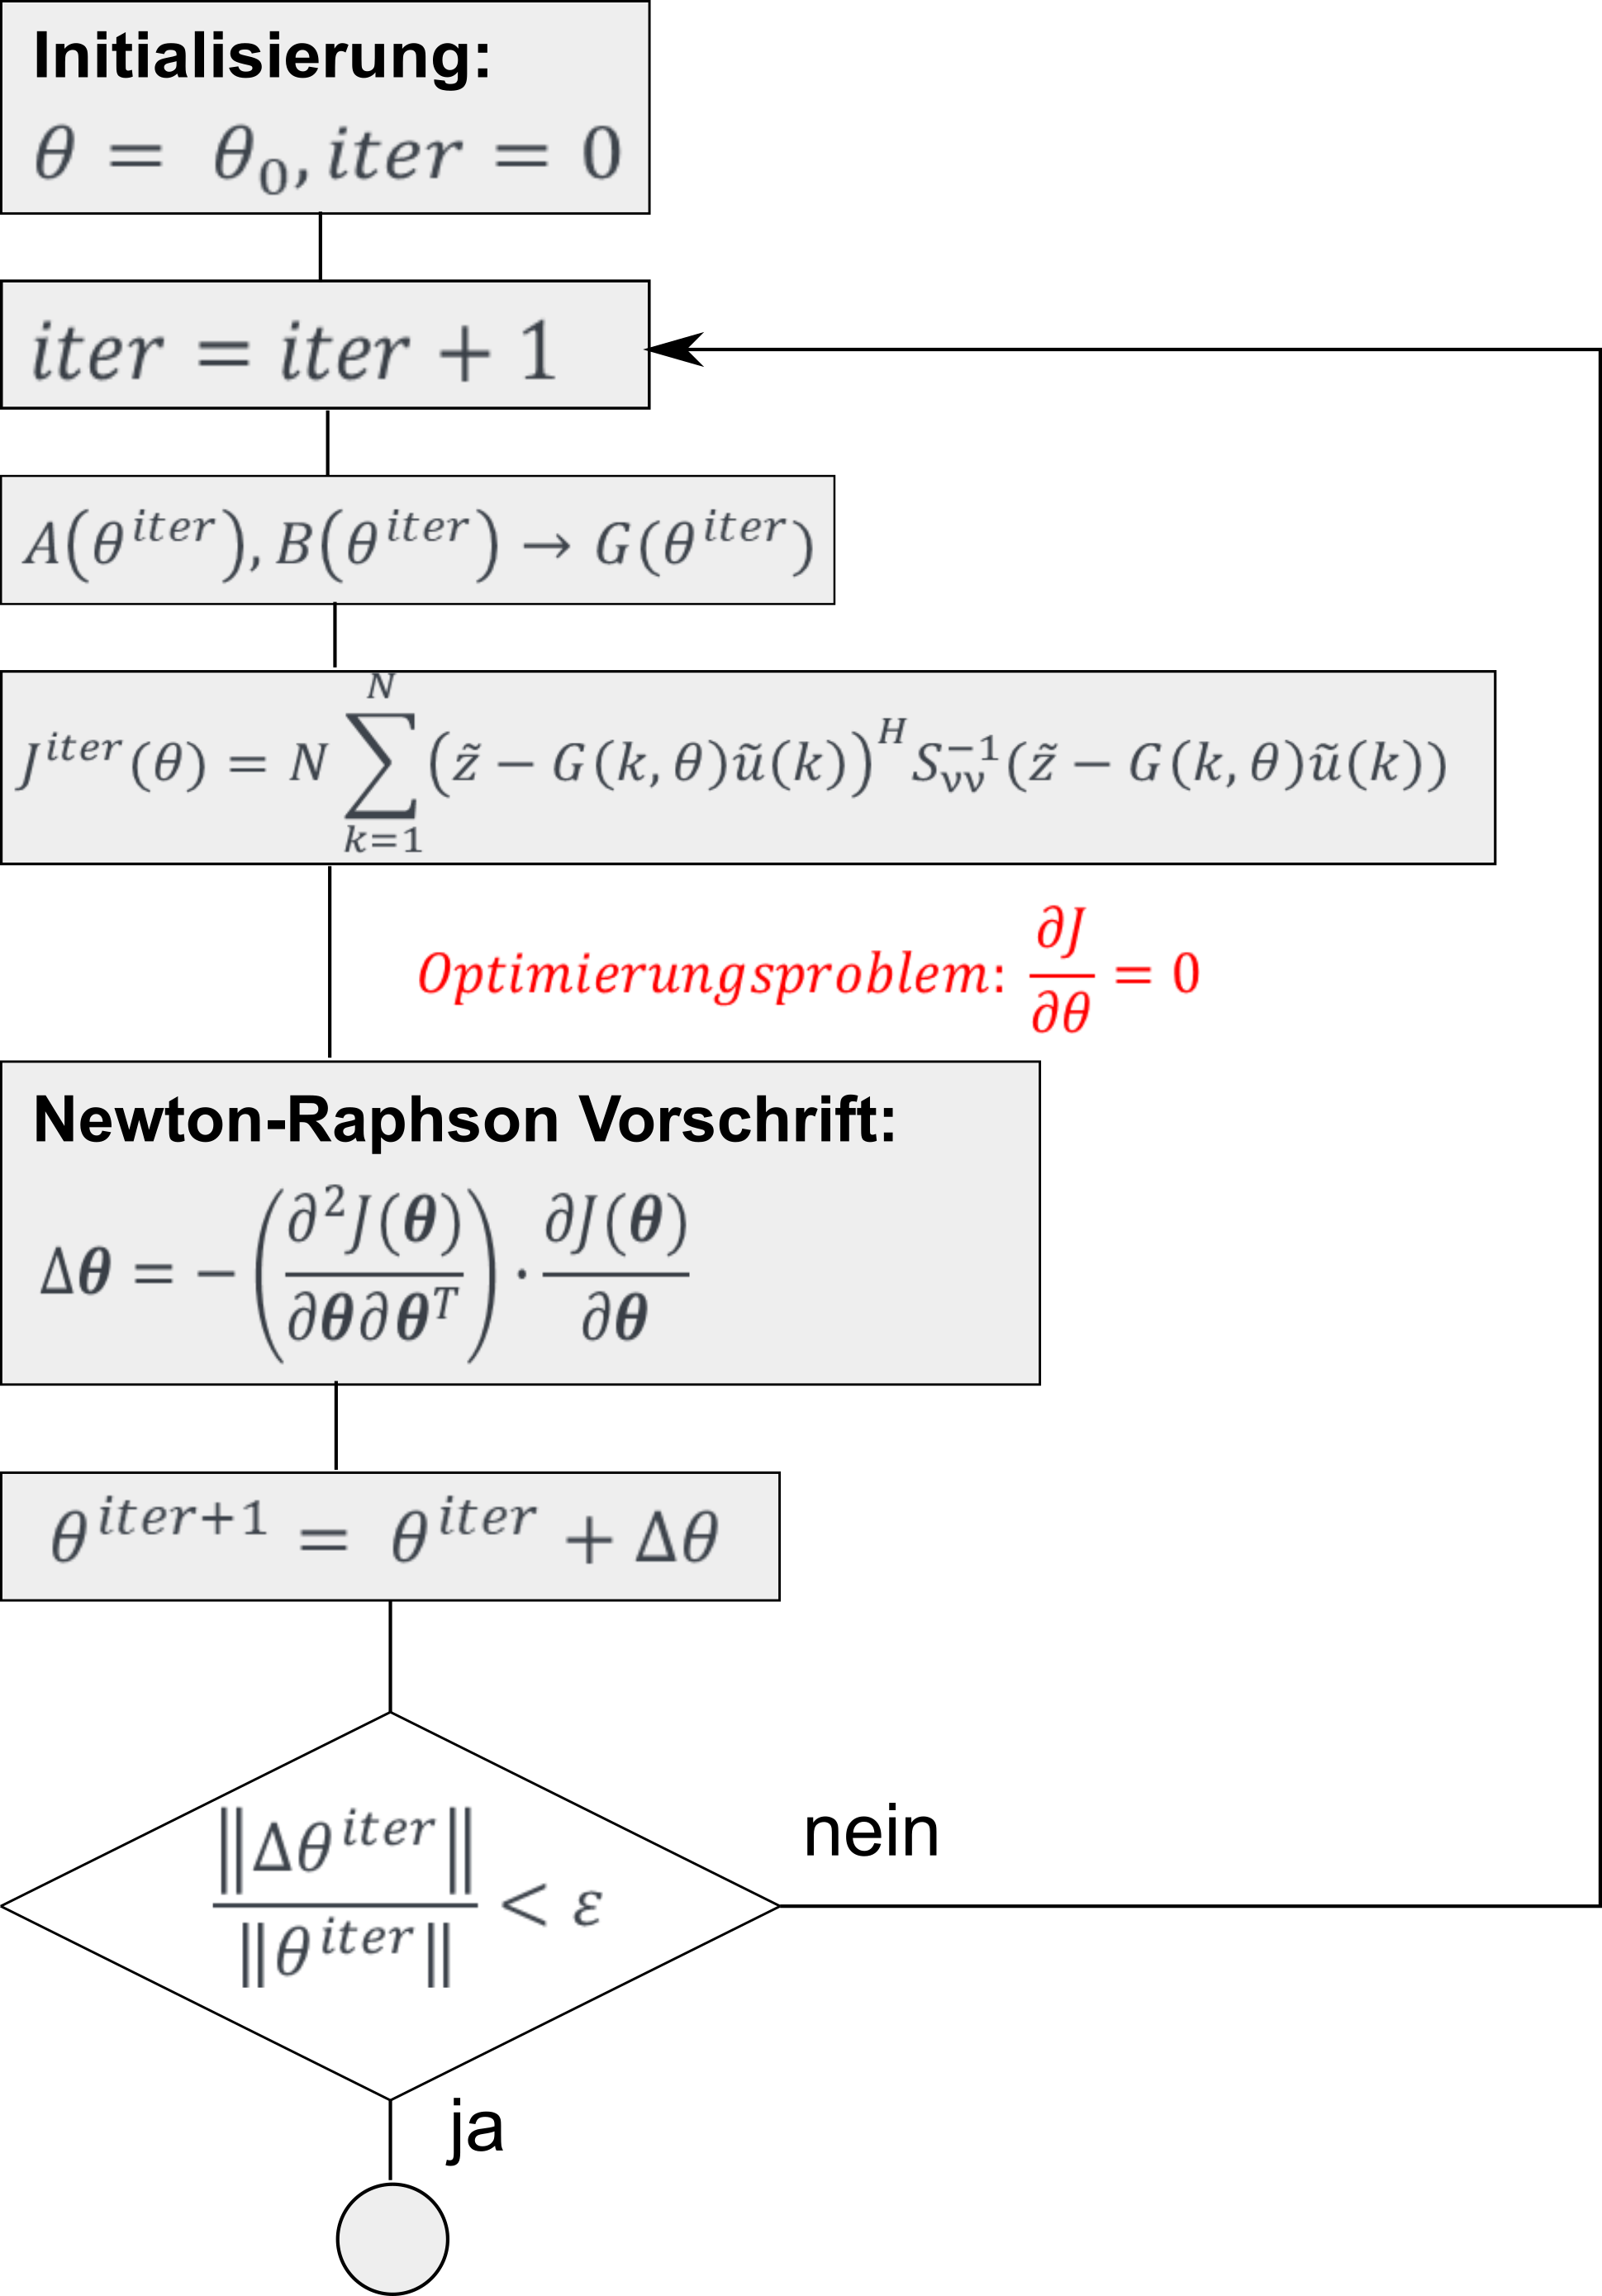
\includegraphics[width=0.6\linewidth]{Newton_Raphson.png}
	\caption{Newton-Raphson Algorithmus für die OEM.}
	\label{fig:Newton_Raphson}
\end{figure}

\section{Vor- und Nachteile}
Wie bereits erwähnt werden bei der Systemidentifikation im Frequenzbereich fouriertransformierte Signalverläufe betrachtet. 
Ein großer Vorteil besteht nun darin, dass die in der Identifikation berücksichtigten Frequenzpunkte frei gewählt werden 
können. Dies ist von Vorteil, wenn im Vorhinein bereits bekannt ist, welche Frequenzen für das Modell eine wichtige Rolle 
spielen. Auch wenn die Berechnungen im Algorithmus durchaus sehr aufwändig werden können, so ist der Rechenaufwand unabhängig 
von der Länge des betrachteten Zeitraums bzw. der Anzahl der Datenpunkte im Zeitbereich.

Darüberhinaus lässt sich ein physikalisches Verständnis des Systems im Frequenzbereich gewinnen, was für viele Anwendungen 
sehr hilfreich sein kann. Im Reglerentwurf beispielsweise sind Frequenzverläufe von großer Wichtigkeit.\\

Ein schwerwiegender Nachteil ist die Notwendigkeit eines passenden Eingangssignals zum Erreichen einer guten Identifikation. 
Als Beispiel sei ein Frequency Sweep, auch Chirp-Signal genannt, bei welchem eine Schwingung mit steigender Frequenz auf eine 
Steuerung gegeben wird. Mit solchen passenden Steuerungen ist mit deutlich besseren Identifikationsergebnissen zu rechnen.

Die Bestimmung der einfachen und zweifachen Ableitungen für die Jacobi- und Hesse-Matrizen ist sehr aufwändig. In diesem 
Projekt wurde deshalb auf die Möglichkeit des symbolischen Rechnens in Matlab zurückgegriffen. Trotdzem bleibt dies ein 
Nachteil.

Schließlich bleibt noch die Berücksichtigung des Abtasttheorems nach Shannon ein wichtiger Punkt, um Frequenzverfälschungen 
zu vermeiden \cite{Grimm2017}. Demzufolge muss die Abtastfrequenz mehr als doppelt so groß sein wie die größte Frequenz im 
Signal. Dies stellte sich bei den vorliegenden Daten jedoch nicht als Problem heraus.

\section{Ergebnisse}

Abschließend will das folgende Kapitel noch einen kurzen Einblick in die Ergebnisse der Parameterschätzung im Frequenzbereich geben. In Abbildung \ref{fig:Ergebnisse_f} sind sowohl die geschätzten Frequenzverläufe als auch die originalen Frequenzverläufe dargestellt. Beim Blick auf die originalen Daten (in Rot dargestellt) fällt der erwartete Trend ins Auge. Die Übertragung findet hauptsächlich im Bereich niedriger Frequenzen statt. Die Verläufe knicken für große Frequenzen ab. Ausnahme ist die Nickrate $q$. Da wir allerdings nur die Bewegung während der Platzrunde betrachten liegt $q$ nahe bei 0 und wird hauptsächlich vom Messrauschen bestimmt. Dies könnte den Anstieg bei hohen Frequenzen erklären. Um ein besserer Bild vom Übertragungsverhalten von $q$ zu bekommen müsste beispielsweiße im Bereich der Anstellwinkelschwingung geflogen werden. Aus dem Newton-Raphson Algorithmus erhält man eine Abschätzung des Parametervektors $\theta$ und damit auch eine Abschätzung der Übertragungsmatrix $G(\theta)$. Mithilfe von $G(\theta)$ und den gemessenen Steuergrößen lässt sich ein geschätzter Frequenzverlauf der Zustandsgrößen berechnen. Dieser ist ebenfalls in Abb. \ref{fig:Ergebnisse_f} eingezeichnet. Es zeigt sich, dass die Frequenzverläufe im Allgemeinen gut getroffen werden. Teilweise werden Ausschläge sogar exakt getroffen (siehe Verlauf von $q$ im niedrigen Frequenzbereich). Das häufigstes Problem, das wir beobachten konnten, war allerdings das Überschätzen bzw. Unterschätzen der Ausgangsverläufe. Deutlich zu sehen ist das im Verlauf der Geschwindigkeit $V_{A}$. Ein Grund könnten die unterschiedlichen Größenordnungen der Zustandsgrößen sein. Dies würde erklären warum die Geschwindigkeit, mit der größten nominellen Abweichung vom Trimmpunkt, unterschätzt wird. Eine Normalisierung der Zustandsgrößen wäre deshalb ein möglicher Ansatz zur Verbesserung der Ergebnisse (siehe Kapitel \ref{chapter:Zusammenfassung}). 

\begin{figure}[h!]
	\centering
	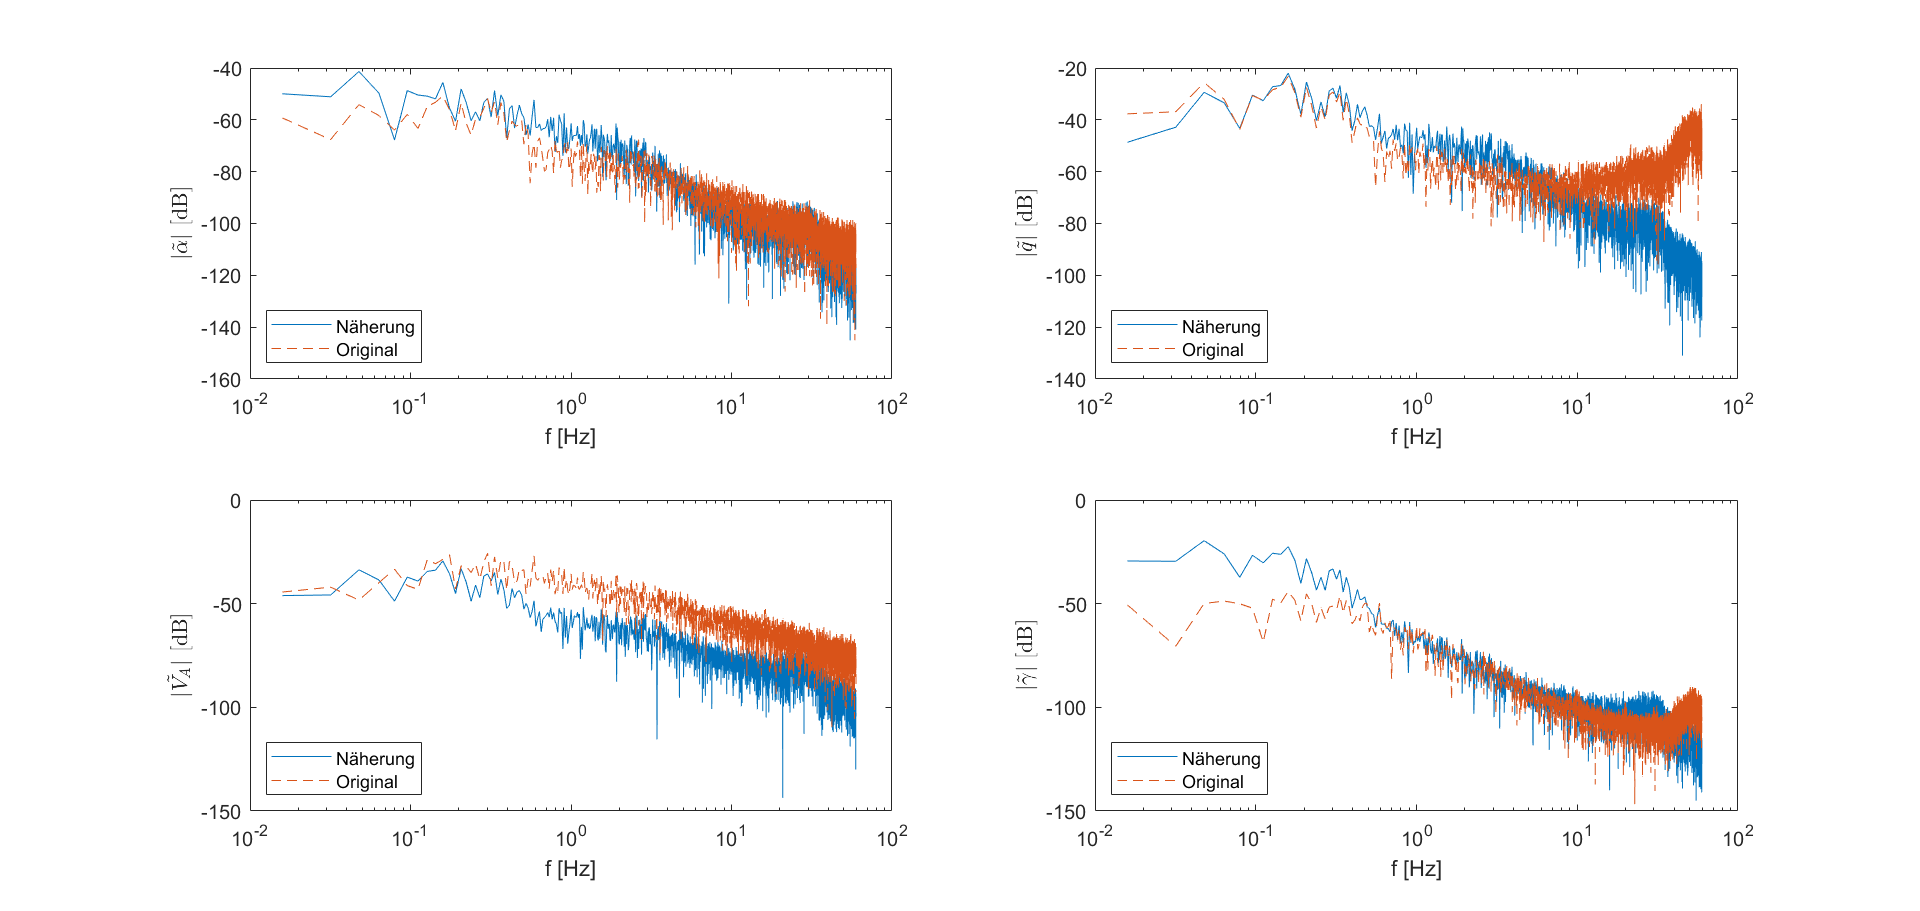
\includegraphics[trim=100 0 100 0,clip,width=1\linewidth]{Ergebnisse_Frequenzbereich.png}
	\caption{Frequenzverläufe der vier Zustandsgrößen der Längsbewegung. In Rot sind die Frequenzverläufe der Messdaten und in Blau die Frequenzverläufe des geschätzten Modells dargestellt.}
	\label{fig:Ergebnisse_f}
\end{figure}

Exemplarisch wurde der Frequenzverlauf des Anstellwinkels $\alpha$ wieder in den Zeitbereich zurück transformiert. Das Ergebnis ist in Abbildung \ref{fig:Ergebnisse_t} dargestellt. Zusätzlich sind die Steuerverläufe von Elevator und Schub aufgetragen. Es ist gut zu erkennen das sogar die Ausschläge im Anstellwinkel abgeschätzt werden und der geschätzte Verlauf ein brauchbares Ergebnis liefert. Weniger realistisch sind allerdings die geschätzten Matrizen des Zustandsraummodells $A$ und $B$. Auch die Verläufe der anderen Größen werden nicht ganz so gut angenähert. Das Problem könnte hier bereits vor der Anwendung des Algorithmus liegen. Die gegebenen Flugdaten sind speziell für ein Schätzverfahren im Frequenzbereich unzureichend. Es ist vor allem interessant in welchem Frequenzbereich ein Steuereingang auf die Zustandsgrößen übertragen wird. Dies erkennt man dann wenn die Frequenzen, beipsielsweise in einem \textit{Frequency Sweep}, abgeflogen werden. Dies wäre eine mögliche Erklärung für die weniger guten Ergebnisse einiger Abschätzungen.

\begin{figure}[h!]
	\centering
	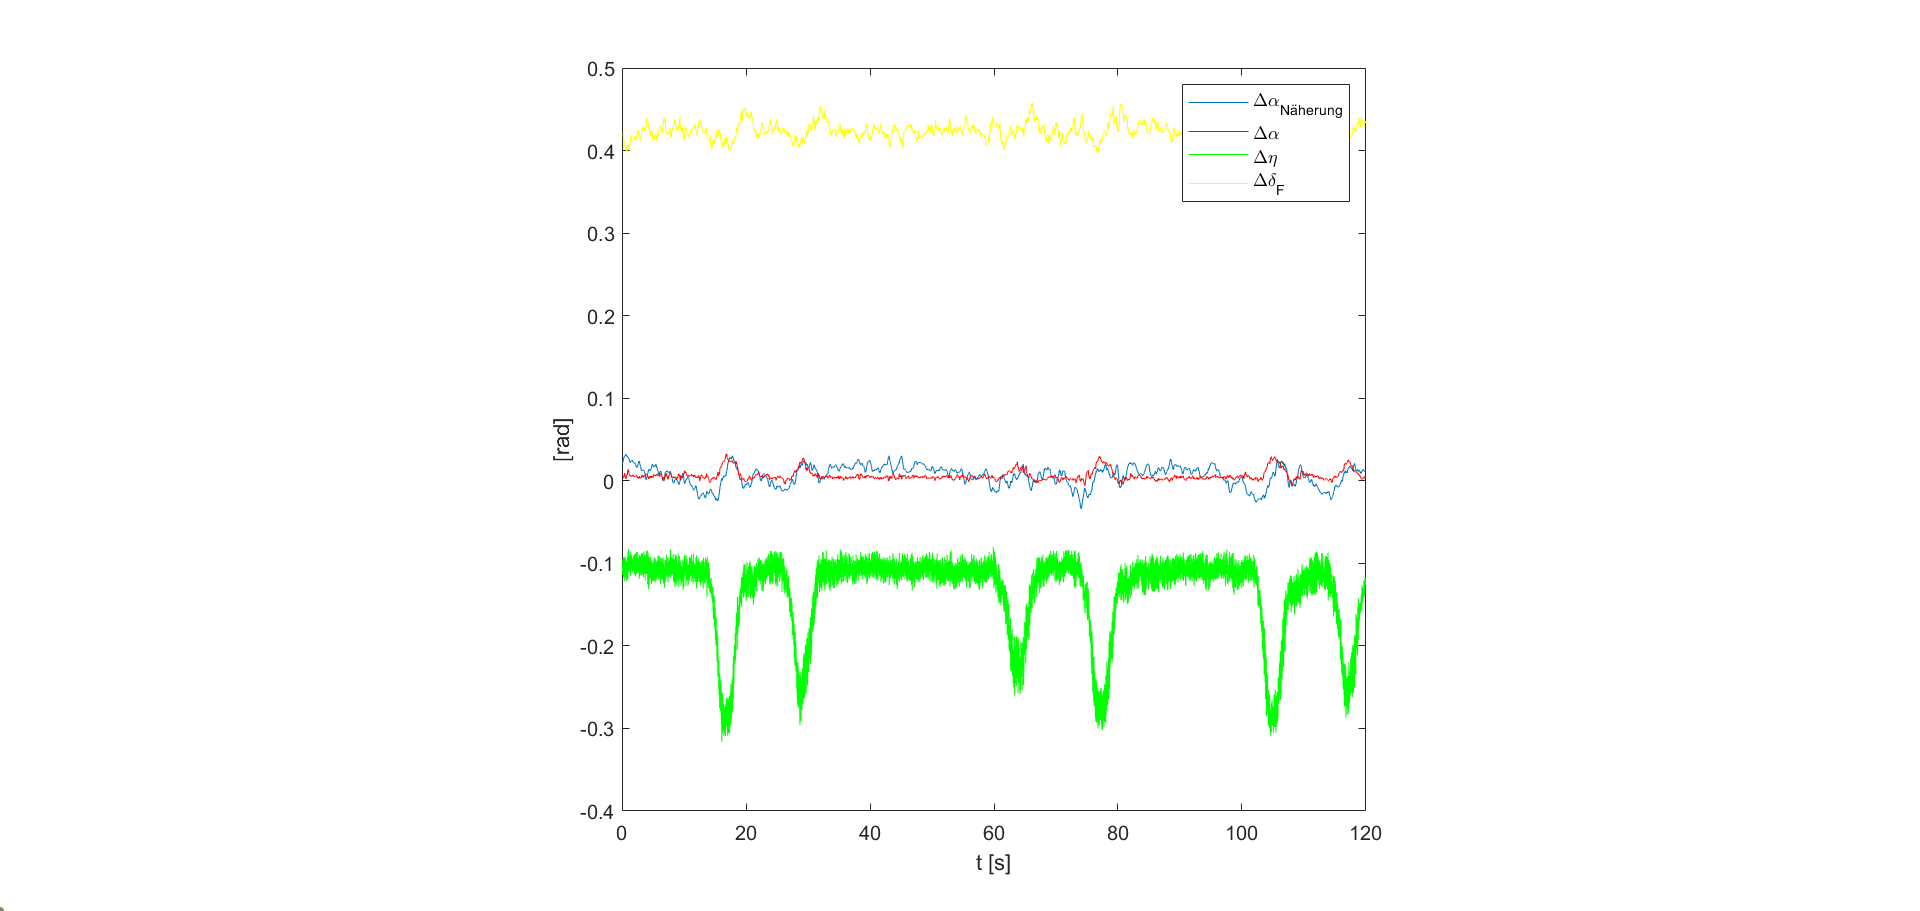
\includegraphics[trim=100 0 100 0,clip,width=1\linewidth]{Ergebnisse_alpha_inv.png}
	\caption{Zeitverlauf der Steuergrößen und der Zustandsgröße $\alpha$.}
	\label{fig:Ergebnisse_t}
\end{figure}